% !TEX TS-program = XeLaTeX
% use the following command:
% all document files must be coded in UTF-8
\documentclass[portuguese]{textolivre}
% build HTML with: make4ht -e build.lua -c textolivre.cfg -x -u article "fn-in,svg,pic-align"

\journalname{Texto Livre}
\thevolume{19}
%\thenumber{1} % old template
\theyear{2026}
\receiveddate{\DTMdisplaydate{2026}{6}{19}{-1}} % YYYY MM DD
\accepteddate{\DTMdisplaydate{2026}{6}{20}{-1}}
\publisheddate{\DTMdisplaydate{2026}{10}{19}{-1}}
\corrauthor{Marcus de Souza Araujo}
\articledoi{10.1590/1983-3652.2026.66782}
%\articleid{NNNN} % if the article ID is not the last 5 numbers of its DOI, provide it using \articleid{} commmand 
% list of available sesscions in the journal: articles, dossier, reports, essays, reviews, interviews, editorial
\articlesessionname{reviews}
\runningauthor{Araujo} 
%\editorname{Leonardo Araújo} % old template
\sectioneditorname{Daniervelin Pereira~\orcid{0000-0003-1861-3609}}
\layouteditorname{Leonardo Araújo~\orcid{0000-0003-3884-2177}}

\title{Resenha do livro Generative Artificial Intelligence: What Everyone Needs to Know}
\othertitle{Review of Generative Artificial Intelligence: What Everyone Needs to Know}
% if there is a third language title, add here:
%\othertitle{Artikelvorlage zur Einreichung beim Texto Livre Journal}

\author[1]{Marcus de Souza Araújo~\orcid{0000-0001-5403-0879}\thanks{Email: \href{mailto:marcusaraujo@ufpa.br}{marcusaraujo@ufpa.br}}}
\affil[1]{Universidade Federal do Pará, Faculdade de Letras
Estrangeiras Modernas, Programa de Pós-Graduação Criatividade e
Inovação em Metodologias de Ensino Superir, Belém, PA, Brasil.}

\addbibresource{article.bib}
% use biber instead of bibtex
% $ biber article

% used to create dummy text for the template file
\definecolor{dark-gray}{gray}{0.35} % color used to display dummy texts
\usepackage{lipsum}
\SetLipsumParListSurrounders{\colorlet{oldcolor}{.}\color{dark-gray}}{\color{oldcolor}}

% used here only to provide the XeLaTeX and BibTeX logos
\usepackage{hologo}

% if you use multirows in a table, include the multirow package
\usepackage{multirow}

% provides sidewaysfigure environment
\usepackage{rotating}

\usepackage{endnotes} % Inclui o pacote endnotes

% CUSTOM EPIGRAPH - BEGIN 
%%% https://tex.stackexchange.com/questions/193178/specific-epigraph-style
\usepackage{epigraph}
\renewcommand\textflush{flushright}
\makeatletter
\newlength\epitextskip
\pretocmd{\@epitext}{\em}{}{}
\apptocmd{\@epitext}{\em}{}{}
\patchcmd{\epigraph}{\@epitext{#1}\\}{\@epitext{#1}\\[\epitextskip]}{}{}
\makeatother
\setlength\epigraphrule{0pt}
\setlength\epitextskip{0.5ex}
\setlength\epigraphwidth{.7\textwidth}
% CUSTOM EPIGRAPH - END

% to use IPA symbols in unicode add
%\usepackage{fontspec}
%\newfontfamily\ipafont{CMU Serif}
%\newcommand{\ipa}[1]{{\ipafont #1}}
% and in the text you may use the \ipa{...} command passing the symbols in unicode

% LANGUAGE - BEGIN
% ARABIC
% for languages that use special fonts, you must provide the typeface that will be used
% \setotherlanguage{arabic}
% \newfontfamily\arabicfont[Script=Arabic]{Amiri}
% \newfontfamily\arabicfontsf[Script=Arabic]{Amiri}
% \newfontfamily\arabicfonttt[Script=Arabic]{Amiri}
%
% in the article, to add arabic text use: \textlang{arabic}{ ... }
%
% RUSSIAN
% for russian text we also need to define fonts with support for Cyrillic script
% \usepackage{fontspec}
% \setotherlanguage{russian}
% \newfontfamily\cyrillicfont{Times New Roman}
% \newfontfamily\cyrillicfontsf{Times New Roman}[Script=Cyrillic]
% \newfontfamily\cyrillicfonttt{Times New Roman}[Script=Cyrillic]
%
% in the text use \begin{russian} ... \end{russian}
% LANGUAGE - END

% EMOJIS - BEGIN
% to use emoticons in your manuscript
% https://stackoverflow.com/questions/190145/how-to-insert-emoticons-in-latex/57076064
% using font Symbola, which has full support
% the font may be downloaded at:
% https://dn-works.com/ufas/
% add to preamble:
% \newfontfamily\Symbola{Symbola}
% in the text use:
% {\Symbola }
% EMOJIS - END

% LABEL REFERENCE TO DESCRIPTIVE LIST - BEGIN
% reference itens in a descriptive list using their labels instead of numbers
% insert the code below in the preambule:
%\makeatletter
%\let\orgdescriptionlabel\descriptionlabel
%\renewcommand*{\descriptionlabel}[1]{%
%  \let\orglabel\label
%  \let\label\@gobble
%  \phantomsection
%  \edef\@currentlabel{#1\unskip}%
%  \let\label\orglabel
%  \orgdescriptionlabel{#1}%
%}
%\makeatother
%
% in your document, use as illustraded here:
%\begin{description}
%  \item[first\label{itm1}] this is only an example;
%  % ...  add more items
%\end{description}
% LABEL REFERENCE TO DESCRIPTIVE LIST - END


% add line numbers for submission
%\usepackage{lineno}
%\linenumbers

\begin{document}
\maketitle

\begin{figure}[htbp]
\centering
\begin{minipage}{.5\textwidth}
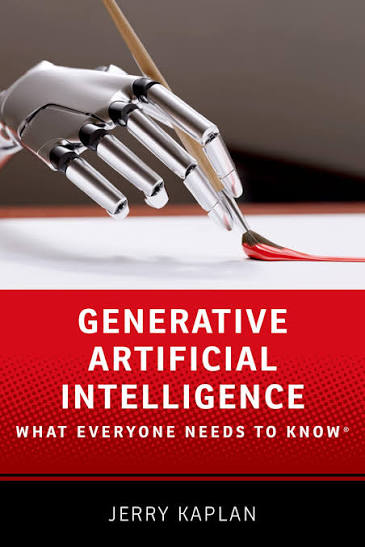
\includegraphics[width=\textwidth]{Fig1.png}
 \caption*{\fullcite{kaplan2024generative}}
 \label{fig01}
\end{minipage}
\end{figure}

\begin{polyabstract}
\begin{abstract}
A resenha avalia a obra \citetitle{kaplan2024generative}, de Jerry Kaplan, a partir de uma discussão sobre a inteligência artificial generativa (IAGen) e sua relevância no cenário contemporâneo, com ênfase em seus desdobramentos éticos, legais e sociais. A obra destaca como os avanços da IAGen têm impulsionado o desenvolvimento de uma nova geração de sistemas computacionais capazes de executar, com elevado grau de desempenho, tarefas tradicionalmente associadas às capacidades humanas. Ao longo da análise, evidencia-se a contribuição de Kaplan (2024) para uma compreensão crítica dessa tecnologia, situando a IAGen como um desafio de natureza civilizatória, cujo enfrentamento requer não apenas avanços técnicos, mas também compromisso ético, responsabilidade social e reflexão coletiva sobre seus impactos.

\keywords{Inteligência artificial \sep Sistemas computacionais \sep Ética \sep Responsabilidade social}
\end{abstract}

\begin{english}
\begin{abstract}
The review evaluates the book \citetitle{kaplan2024generative}, by Jerry Kaplan, through the lens of generative artificial intelligence (GenAI) and its relevance in the contemporary context, with particular emphasis on its ethical, legal, and social implications. The book highlights how advances in GenAI have fostered the development of a new generation of computational systems capable of performing, with a high degree of proficiency, tasks traditionally associated with human capabilities. Throughout the analysis, the review emphasizes the author’s contribution to a critical understanding of this technology, positioning GenAI as a civilizational challenge whose response requires not only technological advancement but also ethical commitment, social responsibility, and collective reflection on its impacts.

\keywords{Artificial intelligence \sep Computational systems \sep Ethics \sep Social responsibility}
\end{abstract}
\end{english}
% if there is another abstract, insert it here using the same scheme
\end{polyabstract}

\section{Introdução}\label{sec-intro}
As mudanças potencializadas pela inteligência artificial generativa (IAGen) na sociedade são latentes na contemporaneidade. Essa tecnologia amplifica a interação entre pessoas e máquinas, proporcionando, em alguns momentos, similaridades e aproximações entre o real e o virtual. A obra \citetitle{kaplan2024generative}, publicada em 2024, pela Editora Oxford, reúne nove capítulos e uma introdução que apresentam um panorama para entender o que é a inteligência artificial generativa e sua importância para os tempos atuais, com discussões também sobre os aspectos éticos, legais e sociais dessa tecnologia. O livro insere-se na série \textit{What everyone needs to know}, da Editora Oxford, apresentando a temática de maneira clara e objetiva, com linguagem acessível a todos os leitores interessados no assunto.

O autor da obra, Jerry Kaplan, é especialista em inteligência artificial, empreendedor, inovador tecnológico, educador e autor de livros. Ele inventou diversas tecnologias inovadoras e fundou inúmeras \textit{startups} de tecnologia. Atualmente, é professor adjunto na Universidade de Stanford, nos Estados Unidos, onde leciona sobre o impacto social e econômico da inteligência artificial.

Embora trate de temas tecnológicos, a obra em tela privilegia uma abordagem explicativa, não técnica, sobre os estudos da IAGen. \textcite{kaplan2024generative} apresenta, de modo compreensível para leitores não especializados, conceitos dos grandes modelos de linguagem e outros fundamentos da inteligência artificial generativa. O público-alvo da obra abrange estudantes dos cursos de licenciatura e pedagogia interessados na temática, gestores preocupados com as implicações éticas, legais e socioeconômicas da inteligência artificial, formuladores de políticas públicas que buscam fundamentos conceituais para o debate sobre regulação tecnológica, além de professores interessados nas práticas sociais mediadas pela IAGen.

\section{Desenvolvimento e análise crítica}\label{sec-normas}
O livro se destaca por apresentar os avanços da inteligência artificial generativa (IAGen) que têm possibilitado o desenvolvimento de uma nova classe de sistemas computacionais capazes de desempenhar, com elevada proficiência, por vezes superior à humana, uma ampla gama de tarefas. Esses sistemas tecnológicos produzem textos, imagens, composições musicais e códigos computacionais inéditos, a partir da análise de vastos volumes de dados digitalizados.

O livro também destaca que, atualmente, tais tecnologias já são aplicadas a atividades mais elaboradas, como, por exemplo, apoio ao atendimento médico especializado, consultoria jurídica, redação de documentos, desenvolvimento de \textit{softwares} e oferta de tutoria personalizada, além da criação artística e musical. Embora esses avanços tenham potencial para acelerar de maneira significativa o progresso científico, artístico e intelectual, também eles instauram novos desafios e riscos que demandam avaliação crítica e regulamentação apropriadas.

Por essa razão, \textcite{kaplan2024generative} ressalta que a inteligência artificial generativa tem desafiado de forma contundente os fundamentos de nosso senso de identidade, ao questionar pressupostos historicamente associados à singularidade humana. A ideia de singularidade apontada por \textcite{kaplan2024generative} é mais que importante no campo da IAGen e na sociedade contemporânea. De acordo com o autor, a singularidade pode ser compreendida como o estágio em que a inteligência artificial adquire a capacidade de promover seu próprio aprimoramento ou de gerar sistemas intelectualmente superiores de maneira autônoma, desencadeando um ciclo acelerado de desenvolvimento tecnológico e cognitivo, cujas consequências podem ser de difícil previsibilidade e controle.

O ritmo de avanço tecnológico seria tão acelerado que os seres humanos não conseguiriam acompanhá-lo, resultando em transformações sociais, econômicas e culturais de grande magnitude, caracterizadas por alto grau de imprevisibilidade. Nessa linha, \textcite{kaplan2024generative} enfatiza que a IAGen mudará praticamente tudo. Em outras palavras, a forma como vivemos, trabalhamos, nos divertimos, nos expressamos, persuadimos uns aos outros, buscamos um parceiro, cuidamos de nossos idosos e educamos nossos jovens, os nativos algoritmos \cite{jorge2025iai}. Segundo essa autora, “eles não vão ‘começar a usar’ a IA; eles vão nascer com ela presente, invisível e constante” \cite[p.~189]{jorge2025iai}.

A obra de \textcite{kaplan2024generative} está organizada em oito capítulos, além da introdução e de uma seção final denominada de \textit{outroduction}, que funciona como um posfácio. Cada seção dos capítulos é organizada a partir de problematizações que, além de estimular a reflexão acerca das perguntas e respostas apresentadas pelo autor, contribuem para uma compreensão mais abrangente do funcionamento da IAGen. Tal abordagem confere à obra um caráter dialógico, alinhando-se a práticas pedagógicas que promovem o pensamento crítico e a autonomia cognitiva do leitor. Ao formular questões que desafiam conceitos consolidados, \textcite{kaplan2024generative} estabelece um espaço de debate que transcende a exposição teórica e engaja o leitor na construção ativa do sentido do texto.

No capítulo da introdução, \textcite{kaplan2024generative} apresenta ao leitor o surgimento e a importância da IAGen no cenário tecnológico contemporâneo, explicando por que essa tecnologia é diferente de versões anteriores de IA e por que ela está acontecendo agora. O autor apresenta um panorama geral sobre como a IAGen pode gerar textos, imagens, músicas, \textit{softwares} e outros conteúdos, transformando a maneira como as pessoas vivem e trabalham na contemporaneidade. \textcite{kaplan2024generative} levanta questões centrais que orientam a obra, como os potenciais benefícios, os riscos, os desafios éticos, os impactos econômicos e as implicações sociais da IAGen. O objetivo principal da introdução é preparar o leitor para a análise crítica que se segue nos capítulos seguintes, destacando que a IAGen não é apenas uma tecnologia, mas um fenômeno social.

As ideias de \textcite{kaplan2024generative} coadunam com as de \textcite[p.~146]{kenski2026tempos} ao salientar que

\begin{quote}
    A IA é mais do que uma ferramenta, […]. Na cultura do digital, ela é um agente cultural, que cria novas manifestações culturais por meio de algoritmos que geram textos, imagens, músicas e até roteiros de filmes. Para isso, a IA absorve e reproduz todas as produções a que tem acesso.
\end{quote}

No primeiro capítulo, \textit{A história da inteligência artificial}, apresenta-se o percurso histórico da IA desde suas origens até o advento das abordagens contemporâneas que possibilitaram o desenvolvimento da IAGen. O autor examina a evolução dessa área do conhecimento em expansão, retomando as formulações iniciais acerca de máquinas inteligentes e avançando pelas contribuições do aprendizado de máquina e das redes neurais artificiais. De modo geral, o capítulo oferece uma fundamentação histórica e conceitual consistente, permitindo compreender as razões pelas quais as tecnologias atuais se distinguem das anteriores em termos de potencialidades e capacidade de transformação.

No segundo capítulo, \textit{Inteligência artificial generativa}, \textcite{kaplan2024generative} discute criticamente o conceito de IAGen, apresentando sua definição, seus princípios de funcionamento e seus modelos computacionais que a viabilizam, como os grandes modelos de linguagem e as redes neurais profundas. O autor explicita, ainda, de que modo esses sistemas são capazes de produzir diferentes tipos de conteúdo, como, por exemplo, textos, imagens, músicas e códigos de programação, enfatizando o papel das bases de dados e do aprendizado profundo nesse processo. O capítulo, outrossim, estabelece distinções entre a IAGen e outras modalidades de automação, contribuindo para uma compreensão mais precisa de suas especificidades e seus alcances.

No terceiro capítulo, \textit{Impactos prováveis}, o autor do livro examina os efeitos potenciais da IAGen em diferentes setores da sociedade e da economia, tais como saúde, educação, criatividade, ciência, negócios e serviços profissionais, incluindo medicina, direito e engenharia de \textit{software}. O capítulo evidencia, ainda, o papel da IAGen na aceleração da produtividade e da inovação, discutindo como essa tecnologia pode transformar esses setores, bem como os grupos que tendem a ser beneficiados ou potencialmente prejudicados pelas mudanças por elas desencadeadas. \textcite{kaplan2024generative} adota uma perspectiva prospectiva, articulada a uma reflexão crítica sobre as incertezas inerentes aos novos modelos de interação entre humanos e tecnologias.

No quarto capítulo, \textit{O futuro do trabalho}, \textcite{kaplan2024generative} problematiza como os processos de automação associados à adoção da IAGen podem reconfigurar o mercado de trabalho, especialmente em tarefas cognitivas, com implicações para a redefinição de profissões, a transformação de ocupações existentes e o surgimento de novas funções. O autor também aborda temas como produtividade, ampliação de desigualdades e necessidade de adaptação das competências humanas diante da crescente automação. O capítulo, por fim, apresenta reflexões sobre as oportunidades e os desafios decorrentes dessas transformações.

No quinto capítulo, \textit{Riscos e perigos}, \textcite{kaplan2024generative} examina os principais desafios decorrentes da difusão da IAGen, destacando questões como vieses algorítmicos, vulnerabilidades de segurança, propagação de desinformação e outras implicações éticas e sociais associadas à tomada de decisões automatizadas e à compatibilidade com valores humanos. O autor também ressalta o caráter potencialmente transformador dessa tecnologia, enfatizando a necessidade para a elaboração de estratégias e políticas públicas capazes de mitigar riscos sem, contudo, comprometer os benefícios e as oportunidades que dela podem advir.

No sexto capítulo, \textit{Os status legais das IAGens}, o autor analisa os desafios jurídicos decorrentes do uso das IAGens, especialmente no que se refere à propriedade intelectual dos conteúdos produzidos, à responsabilidade por decisões automatizadas e aos direitos sobre criações originárias dessas tecnologias. Discute-se, ainda nesse capítulo, de que modo a legislação vigente contempla, ou deixa de contemplar, situações envolvendo danos causados por aplicações de IAGen e a dificuldade de enquadrar juridicamente entidades que geram resultados criativos sem intervenção humana direta. \textcite{kaplan2024generative} destaca a urgência de fóruns e mecanismos regulatórios capazes de revisar e atualizar os marcos normativos, uma vez que grande parte das leis atuais se mostra desatualizada para tratar adequadamente as especificidades introduzidas por esses novos agentes tecnológicos.

No sétimo capítulo, \textit{Regulamentação, política pública e competição global}, \textcite{kaplan2024generative} discute a necessidade de marcos regulatórios e políticas públicas capazes de orientar o uso da IAGen, de modo a conciliar estímulo à inovação com medidas de precaução. O autor analisa diferentes estratégias adotadas por governos para supervisionar e normatizar esta tecnologia, destacando como tais escolhas afetam a competitividade internacional e a configuração das relações entre países que lideram seu desenvolvimento. Examina, ainda, as iniciativas de governança adotadas em distintas regiões e a potencialidade de modelos de cooperação internacional para a mitigação de riscos transnacionais. A conclusão de \textcite{kaplan2024generative} é contundente: decisões regulatórias não apenas definem o acesso às tecnologias de IAGen, mas também reconfiguram a distribuição de poder global, tornando a governança internacional um fator estratégico para o século XXI.

No oitavo capítulo, \textit{Questões filosóficas e implicações}, o autor problematiza os significados de inteligência, criatividade e consciência quando atribuídos a máquinas. \textcite{kaplan2024generative} examina como a IAGen desafia concepções tradicionais de singularidade humana e discute implicações filosóficas mais amplas acerca do papel da tecnologia na sociedade contemporânea. O capítulo ainda destaca as consequências éticas decorrentes das interações entre seres humanos e sistemas que simulam capacidades cognitivas humanas, bem como o impacto dessas relações na compreensão da humanidade e autonomia. Assim sendo, o capítulo em tela evidencia que a questão central não é apenas saber se máquinas podem ser inteligentes ou criativas, mas também como essas atribuições transformam a própria definição de humanidade.

Por fim, o livro encerra-se com a seção intitulada \textit{Outroduction}, na qual são apresentadas as considerações finais da obra. Nela, o autor convida o leitor a refletir criticamente sobre os caminhos que a sociedade deve adotar para orientar o desenvolvimento e o uso da IAGen a favor do bem comum e da sustentabilidade. Esse capítulo reitera a importância de um diálogo qualificado entre especialistas em tecnologia, formuladores de políticas públicas e a sociedade em geral, visando à construção de respostas éticas e sociais adequadas aos desafios emergentes.

\section{Conclusão}\label{sec-conduta}
O livro resenhado \citetitle{kaplan2024generative} reafirma que as decisões tomadas sobre o uso da IAGen na contemporaneidade repercutirão de forma duradoura na configuração das relações humanas e institucionais futuras. Ao convidar para uma reflexão crítica, \textcite{kaplan2024generative} posiciona a IAGen como um desafio de ordem civilizatória, cujo enfrentamento demanda não apenas inovação técnica, mas, principalmente, compromisso ético e responsabilidade social.

Como limitação da obra, destaca-se a ausência de uma discussão mais aprofundada sobre políticas educacionais voltadas ao uso ético e responsável da IAGen, bem como sobre seus letramentos. Embora esses temas sejam centrais para a integração crítica dessa tecnologia aos contextos educacionais, eles não são explorados de maneira específica, o que leva o leitor a recorrer a outras obras para ampliar sua compreensão acerca desses aspectos.

A atualidade dos debates e a relevância das reflexões apresentadas conferem à obra uma leitura indispensável aos profissionais interessados em compreender o papel da inteligência artificial generativa na sociedade contemporânea com ramificações nas diferentes áreas do conhecimento. Cumpre destacar que o livro não pretende esgotar o tema, mas oferecer subsídios analíticos e críticas pertinentes sobre o assunto em questão. Suas discussões mostram-se especialmente valiosas para professores, estudantes, gestores e formuladores de políticas públicas que as adotem como objeto de pesquisa ou insumo potencial para a elaboração de práticas pedagógicas. Esses atores, em particular, são chamados a considerar, de forma equilibrada, tanto as potencialidades dessa tecnologia quanto os riscos, as incertezas e os possíveis efeitos adversos decorrentes de seu uso na sociedade contemporânea.




\printbibliography\label{sec-bib}
% if the text is not in Portuguese, it might be necessary to use the code below instead to print the correct ABNT abbreviations [s.n.], [s.l.]
%\begin{portuguese}
%\printbibliography[title={Bibliography}]
%\end{portuguese}

\section*{\fontsize{10}{12}\selectfont Nota de transparência metodológica}
A presente resenha contou com apoio pontual do ChatGPT em etapas de revisão linguística e de aprimoramento da organização textual. Contudo, a  interpretação analítica, as apreciações críticas e os posicionamentos avaliativos apresentados são de responsabilidade exclusiva do autor, em consonância com os princípios de integridade e ética científica que orientam a produção acadêmica.

\begin{dataavailability}
\txtdataavailability{nodata} % options: dataavailable, dataonly, databody, datanotav, nodata
\end{dataavailability}

\end{document}

